%&"../main"
\documentclass[../main]{subfiles}
\begin{document}

\chapter{外汇分析}%
\label{cha:外汇分析}

\section{外汇管理必要性}%
\label{sec:外汇管理必要性}

由表\ref{tab:华为国内外收入及占比}数据可知,海外收入在公司总收入中占比仍不可小觑
。公司海外业务收入在总收入占比超过半足以证明华为公司跨国经营的程度。随着公司的
扩展,公司受汇率波动影响的范围也逐渐扩大。2017 年,人民币汇率双向波动趋势更加明
显,由于公司主要外币敞口是美元和欧元,因此右图图列示了2017年以来,人民币对美元和
人民币对欧元中间价波动情况,从图中可以看出,进入2017年,人民币对美元和对欧元的汇
率波动弹性增大且双向波动趋势更加明显。面对不同外币汇率变动带来的影响,公司在经营
中应考虑不同甚至截然相反的应对措施,这对公司的外汇风险管理水平提出更高的要求。

\begin{table}[htbp]
	\centering
	\caption{华为国内外收入及占比}
	\label{tab:华为国内外收入及占比}
	\csvautobooktabular{tab/income.csv}
\end{table}

\begin{figure}[htbp]
	\centering
	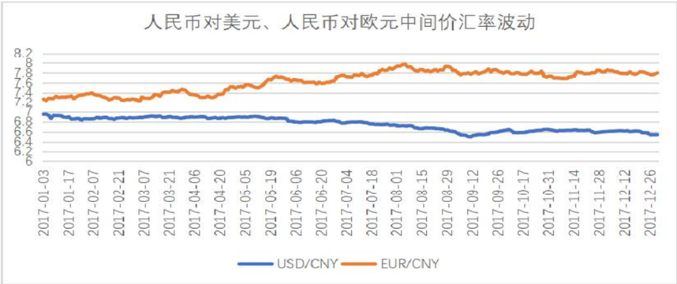
\includegraphics[width = 0.8\linewidth]{money.png}
	\caption{人民币对美元、欧元中间价波动}
	\label{fig:人民币对美元、欧元中间价波动}
\end{figure}

\section{现行外汇管理措施}%
\label{sec:现行外汇管理措施}

公司现有的管理外汇风险的手段如下:

\begin{enumerate}

	\item 管理对外业务合同规避外汇风险;

	\item 管理企业自有资金降低风险端口;

	\item 使用外币借款管理外币风险;

	\item 利用金融衍生工具规避外汇风险;

	\item 建立海外财务公司管理外汇风险;

	\item 进入银行间人民币外汇市场,有效控制外汇风险;

\end{enumerate}

如果想要确定公司外汇风险的效果,需要进一步对公司当前的外汇风险进行评估,下面是外
汇风险的三种类型,主要介绍经济风险。

\begin{table}[htbp]
	\centering
	\caption{外汇风险}
	\label{tab:外汇风险}
	\csvautobooktabular{tab/risk.csv}
\end{table}

\section{经济风险评估}%
\label{sec:经济风险评估}

经济风险对企业产生的影响主要是通过影响企业经营过程中的具体业务进而影响企业的利润
。而由于具体业务的不同,各业务受经济风险影响的程度大小也不同。华为公司的海外收入
主要来源于通讯设备的销售及配套产品的相关服务,汇率变动影响公司具体的业务活动最终
影响公司的利润。右表列示了经济风险给华为公司的日常业务的影响情况。

\begin{table}[htbp]
	\centering
	\caption{经济风险给华为公司的现金流入业务的影响情况}
	\label{tab:经济风险给华为公司的现金流入业务的影响情况}
	\csvautobooktabular{tab/influence.csv}
\end{table}

\begin{table}[htbp]
	\centering
	\caption{经济风险给华为公司的现金流出业务的影响情况}
	\label{tab:经济风险给华为公司的现金流出业务的影响情况}
	\csvautobooktabular{tab/influence.csv}
\end{table}

由于经济风险影响跨度期间较长,要准确计量存在很大的难度,于是我们分析汇率变动对公
司净利润带来的影响来评估华为的经济风险假定其他风险因素不发生变动,仅将汇率作为唯
一风险变量,则华为在2016年末、2015年末及2014年年末使人民币对美元、欧元汇率分别升
值\%将导致公司净利润减少,具体的变动情况在右表中列示,表中金额用财务报表中当年年
末汇率折算成人民币表示。

\begin{table}[htbp]
	\centering
	\caption{人民币对美元、欧元汇率变动对公司影响}
	\label{tab:人民币对美元、欧元汇率变动对公司影响}
	\csvautobooktabular{tab/change.csv}
\end{table}

在上述同样的假设条件下,如果人民币对美元、欧元汇率发生相反变动,即人民币贬值\%,
将产生与上表金额相同但方向相反的计算结果。由上表可以看出,汇率变动对企业净利润影
响很大,如果从外汇风险的角度出发,企业净利润一定程度上也受到汇率变动的影响,以
2016年人民币对美元升值\%为例,人民币升值\%,华为的净利润将下降1.69亿元,占当年利
润的0.4\%。 因此,汇率变动带来的经济风险对华为的经营成果和公司价值产生了相当大程
度的影响。

\section{横向对比}%
\label{sec:横向对比}

中兴通讯与华为处于同一行业,并且两家公司的主营业务及各业务结构相似。在存在大量海
外业务的背景下,华为公司连续三年汇兑损失持续上升。中兴通讯却实现了从净损失逐步降
低到正的净收益的转变。华为虽然实施了一系列的外汇风险管理政策和措施,但外汇风险管
理效果仍然不尽如人意,现行的对外汇风险的管理措施仍然存在不足。

\begin{table}[htbp]
	\centering
	\caption{横向对比}
	\label{tab:横向对比}
	\csvautobooktabular{tab/compare.csv}
\end{table}

\end{document}

